
\documentclass[UTF8,zihao=-4]{ctexart}
\usepackage[a4paper,top=2.35cm,bottom=2.35cm,left=2.35cm,right=2.35cm]{geometry}
\usepackage{fontspec}
\usepackage{xeCJK}
\setmainfont{DejaVu Sans}
\setsansfont{DejaVu Sans}
\setmonofont{Noto Sans Mono}
\setCJKmainfont{Noto Sans CJK SC}
\setCJKsansfont{Noto Sans CJK SC}
\setCJKmonofont{Noto Sans CJK SC}
\usepackage{booktabs}
\usepackage{longtable}
\usepackage{array}
\usepackage{tabularx}
\usepackage{enumitem}
\usepackage{xcolor}
\usepackage{hyperref}
\usepackage{fancyhdr}
\usepackage{titlesec}
\usepackage{lastpage}
\usepackage{pifont}
\usepackage{amsmath}
\usepackage{amssymb}
\usepackage{makecell}
\usepackage{multirow}
\usepackage{tikz}
\usetikzlibrary{arrows.meta,positioning,shapes,fit}
\hypersetup{colorlinks=true,linkcolor=black,urlcolor=blue,citecolor=black}
\definecolor{RuleBlue}{RGB}{25,74,135}
\definecolor{LightBlue}{RGB}{236,243,252}
\definecolor{LightGray}{RGB}{247,247,247}
\definecolor{DarkGray}{RGB}{80,80,80}
\definecolor{WarnOrange}{RGB}{172,103,0}
\definecolor{RejectRed}{RGB}{150,35,35}
\definecolor{PassGreen}{RGB}{38,118,82}
\definecolor{SoftGreen}{RGB}{237,247,241}
\definecolor{SoftYellow}{RGB}{255,248,229}
\titleformat{\section}{\Large\bfseries\color{RuleBlue}}{\thesection}{0.8em}{}
\titleformat{\subsection}{\large\bfseries}{\thesubsection}{0.8em}{}
\titleformat{\subsubsection}{\normalsize\bfseries}{\thesubsubsection}{0.8em}{}
\setlist[itemize]{topsep=3pt,itemsep=2pt,parsep=0pt,leftmargin=1.9em}
\setlist[enumerate]{topsep=3pt,itemsep=2pt,parsep=0pt,leftmargin=2.2em}
\newcolumntype{Y}{>{\raggedright\arraybackslash}X}
\newcolumntype{L}[1]{>{\raggedright\arraybackslash}p{#1}}
\newcommand{\Pass}{\textcolor{PassGreen}{\ding{51}}}
\newcommand{\Warn}{\textcolor{WarnOrange}{\ding{115}}}
\newcommand{\Reject}{\textcolor{RejectRed}{\ding{55}}}
\newcommand{\Code}[1]{\texttt{#1}}
\newcommand{\Term}[1]{\textbf{#1}}
\newenvironment{notebox}[1]{\vspace{0.5em}\noindent\colorbox{LightBlue}{\parbox{0.96\linewidth}{\textbf{#1}}}\par\vspace{-0.2em}\begin{quote}\small}{\end{quote}\vspace{0.3em}}
\newenvironment{decisionbox}[1]{\vspace{0.5em}\noindent\colorbox{LightGray}{\parbox{0.96\linewidth}{\textbf{#1}}}\par\vspace{-0.2em}\begin{quote}\small}{\end{quote}\vspace{0.3em}}
\newenvironment{greenbox}[1]{\vspace{0.5em}\noindent\colorbox{SoftGreen}{\parbox{0.96\linewidth}{\textbf{#1}}}\par\vspace{-0.2em}\begin{quote}\small}{\end{quote}\vspace{0.3em}}
\newenvironment{warnbox}[1]{\vspace{0.5em}\noindent\colorbox{SoftYellow}{\parbox{0.96\linewidth}{\textbf{#1}}}\par\vspace{-0.2em}\begin{quote}\small}{\end{quote}\vspace{0.3em}}

\hypersetup{pdftitle={L3MetricsEngine v2 System Architecture Design}, pdfauthor={ChatGPT for Lingji Qiwuzhi}}
\pagestyle{fancy}
\fancyhf{}
\lhead{L3MetricsEngine v2 Architecture}
\rhead{RDDQF Implementation Blueprint}
\cfoot{第 \thepage\ 页}

\begin{document}

\begin{titlepage}
\centering
\vspace*{2.2cm}
{\Huge\bfseries L3MetricsEngine v2 系统架构设计\par}
\vspace{0.35cm}
{\Large System Architecture Design for Training Data Quality Assessment\par}
\vspace{0.65cm}
{\LARGE v1.0\par}
\vspace{1.2cm}
\begin{tabular}{rl}
文档定位： & RDDQF 理论体系到工程实现之间的核心架构蓝图 \\
适用系统： & 灵机启物机器人数采质检平台 L3 v2 \\
核心目标： & 将 L3 从 Metric Script 升级为 Evidence-driven Quality Engine \\
输入数据： & TeleDex processed 数据，尤其是 telemetry.npz、manifest、metadata \\
输出对象： & Episode Quality Profile、Timeline Evidence、Batch Quality Report \\
后续用途： & 后端重构、缓存设计、API 设计、前端质量画像、数据集发布 \\
\end{tabular}
\vfill
\begin{minipage}{0.88\linewidth}
\centering\large\bfseries
L3MetricsEngine v2 的目标不是继续在 v1 上追加指标，而是建立 Feature Layer - Evidence Layer - Metric Layer - Quality Layer - Decision Layer 的分层质量评价引擎。
\end{minipage}
\vfill
{\large 2026 年 6 月\par}
\end{titlepage}

\tableofcontents
\newpage

\section*{执行摘要}
\addcontentsline{toc}{section}{执行摘要}

本文档定义 L3MetricsEngine v2 的系统架构。它是 RDDQF 理论文档体系进入工程实现之前的最后一份核心设计文档。前置文档已经回答了“为什么评价训练数据”“评价哪些质量维度”“每个质量维度由哪些证据支持”“指标库应如何组织”等问题。本文档进一步回答：这些概念在后端系统中如何分层、如何组织数据流、如何持久化、如何提供 API、如何服务前端人工 QC 和批次数据集报告。

L3 v1 的计算链路可以概括为：从 \Code{telemetry.npz} 读取时序数组，直接计算若干指标，返回指标卡片和 timeline 段。该模式简单直接，但存在三个根本限制：第一，指标和质量语义绑定过紧，导致新增或替换算法时容易破坏输出结构；第二，缺少 Feature 与 Evidence 中间层，导致系统难以解释“为什么这个 episode 质量低”；第三，计算结果没有成为可复用的数据资产，每次打开页面都倾向于重新计算。

L3 v2 的基本范式是：

\begin{verbatim}
TeleDex processed data
      -> Feature Extraction
      -> Evidence Extraction
      -> Metric Computation
      -> Quality Node Scoring
      -> Score Fusion / Decision
      -> Timeline / Report / Cache / UI
\end{verbatim}

在该范式下，指标不再是系统的第一对象，\Term{Quality Node} 和 \Term{Evidence Record} 才是系统的第一对象。算法可以迭代，指标可以替换，但质量本体和证据结构保持稳定。这个架构使 L3 能够从“页面实时算分模块”升级为“机器人训练数据质量基础设施”。

\section{设计目标与边界}

\subsection{设计目标}

L3MetricsEngine v2 的首要目标是服务训练数据筛选，而不是评价机器人控制器本身。它应回答以下问题：

\begin{enumerate}
\item 这条 demonstration 是否提供了足够清晰、连续、可学习的动作信号？
\item 这条数据是否存在会干扰模型学习的运动抖动、长时间无效片段、异常反复修正或观测同步问题？
\item 这条数据的质量问题发生在什么时间段，人工复核时应优先看哪里？
\item 这条数据是否适合进入训练集，是否应降权、截断、修复、复核或剔除？
\item 一批数据整体上是否具有合理的质量分布、多样性和发布条件？
\end{enumerate}

\subsection{非目标}

L3 v2 不直接替代 L2 和 L4。L2 仍主要负责视觉质量，L4 仍主要负责任务完成度的人工判断。L3 v2 可以吸收 L2/L4 的结果作为证据，但不应在第一阶段通过复杂 VLM 自动判断任务成功与否。

L3 v2 也不是低层机器人控制器诊断系统。Command Tracking Error、Effort Spike 等仍可保留为诊断证据，但不应成为训练质量主评分的核心依据。

\begin{notebox}{核心边界}
L3 v2 的评价对象是 demonstration 对下游 policy learning 的价值，而不是机器人硬件、控制器或操作员个人能力的单独表现。
\end{notebox}

\section{从 L3 v1 到 L3 v2 的范式迁移}

\subsection{L3 v1 的结构}

当前 L3 v1 采用单层 Metric Engine 结构：

\begin{verbatim}
telemetry.npz
  -> L3MetricsEngine.compute_all()
  -> metrics[] + Q_motion + timelineSegments[]
\end{verbatim}

其优点是实现简单、可解释性强、对人工 QC 页面友好。但缺点是所有质量概念被压缩到少数指标卡片中，无法区分“特征”“证据”“指标”“质量维度”“最终决策”。

\subsection{L3 v2 的结构}

L3 v2 采用多层结构：

\begin{verbatim}
Data Source
  -> Feature Layer
  -> Evidence Layer
  -> Metric Layer
  -> Quality Layer
  -> Decision Layer
  -> Timeline / Report Layer
\end{verbatim}

每一层都有稳定的数据契约。Feature 是可复用的底层时序特征，Evidence 是支持质量判断的解释性事实，Metric 是对 Evidence 的数值化聚合，Quality 是本体节点上的评分，Decision 是面向训练集准入的处理建议。

\subsection{迁移原则}

\begin{longtable}{L{3.2cm} L{5.1cm} L{5.9cm}}
\toprule
迁移项 & v1 逻辑 & v2 逻辑 \\
\midrule
核心对象 & Metric & Quality Node + Evidence \\
综合分 & Q\_motion & Training Suitability + Dimension Scores \\
Timeline & 异常段 & 异常段 + 低信息段 + 关键学习段 + 复核段 \\
计算方式 & 页面打开实时计算 & 离线优先，按需补算，版本化缓存 \\
阈值 & 经验阈值 & 数据分布 + 任务类型 + 标注反馈 \\
UI 展示 & 指标卡片 & 质量画像、证据树、时间轴证据、同类对比 \\
系统定位 & Motion QC & Training Data Quality Infrastructure \\
\bottomrule
\end{longtable}

\section{总体架构}

\subsection{分层架构图}

\begin{center}
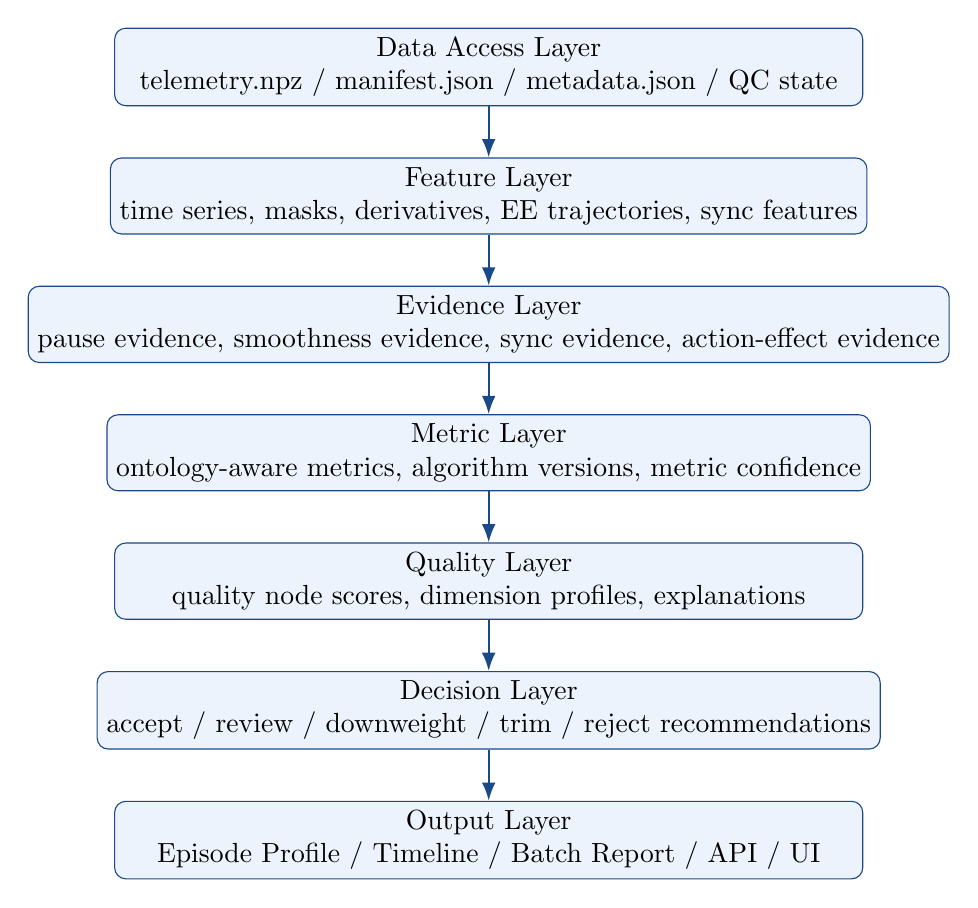
\begin{tikzpicture}[
  node distance=0.65cm,
  box/.style={rectangle,draw=RuleBlue,rounded corners,align=center,minimum width=9.5cm,minimum height=0.72cm,fill=LightBlue},
  arr/.style={-Latex,thick,draw=RuleBlue}
]
\node[box] (data) {Data Access Layer\\telemetry.npz / manifest.json / metadata.json / QC state};
\node[box,below=of data] (feature) {Feature Layer\\time series, masks, derivatives, EE trajectories, sync features};
\node[box,below=of feature] (evidence) {Evidence Layer\\pause evidence, smoothness evidence, sync evidence, action-effect evidence};
\node[box,below=of evidence] (metric) {Metric Layer\\ontology-aware metrics, algorithm versions, metric confidence};
\node[box,below=of metric] (quality) {Quality Layer\\quality node scores, dimension profiles, explanations};
\node[box,below=of quality] (decision) {Decision Layer\\accept / review / downweight / trim / reject recommendations};
\node[box,below=of decision] (report) {Output Layer\\Episode Profile / Timeline / Batch Report / API / UI};
\draw[arr] (data) -- (feature);
\draw[arr] (feature) -- (evidence);
\draw[arr] (evidence) -- (metric);
\draw[arr] (metric) -- (quality);
\draw[arr] (quality) -- (decision);
\draw[arr] (decision) -- (report);
\end{tikzpicture}
\end{center}

\subsection{核心思想}

Engine v2 的核心思想可以概括为三句话：

\begin{enumerate}
\item \Term{Feature 是计算复用层}：所有算法共享同一套基础特征，避免重复读取 MinIO 和重复计算导数、mask、分段。
\item \Term{Evidence 是解释层}：每一个质量判断都必须能回溯到一组证据，而不是只给出一个不可解释分数。
\item \Term{Quality 是业务语义层}：前端、报告、数据库和数据集发布不直接面向算法名称，而面向质量本体节点。
\end{enumerate}

\section{数据输入层}

\subsection{输入文件}

L3 v2 主要依赖 TeleDex processed 数据。输入优先级如下：

\begin{longtable}{L{4cm} L{4cm} L{6cm}}
\toprule
输入 & 用途 & 说明 \\
\midrule
\Code{telemetry.npz} & 核心时序数据 & 包含 qpos、qvel、actions、effort、timestamps、sync、EE pose、IMU 等。 \\
\Code{manifest.json} & 快速元数据 & 提供 fps、duration、frame count、collect depth/tactile/imu 等字段。 \\
\Code{metadata.json} & 对齐和转换信息 & 提供 alignment、sensor offsets、valid time range、conversion 配置。 \\
\Code{camera\_info.json} & 相机标定信息 & 当前阶段主要用于扩展，不作为 L3 motion 计算核心输入。 \\
数据库 Episode 元数据 & 任务上下文 & 包含批次、任务、episode 编号、人工 QC 状态、原因码等。 \\
L2/L4 结果 & 跨层证据 & 可作为 Observation Quality 与 Task Quality 的外部证据。 \\
\bottomrule
\end{longtable}

\subsection{Data Access Layer 职责}

Data Access Layer 应统一负责 MinIO 读取、文件存在性检查、npz 解析、JSON 解析、数据裁剪、dtype 校验和基础异常处理。上层模块不应直接访问 MinIO。

\begin{verbatim}
class EpisodeDataBundle:
    episode_id: int
    telemetry: TelemetryData
    manifest: ManifestData | None
    metadata: MetadataData | None
    episode_meta: EpisodeMeta
    l2_result: Optional[L2Result]
    l4_result: Optional[L4Result]
\end{verbatim}

\subsection{输入校验}

输入校验不直接给训练质量打分，而是决定该 episode 是否可以进入计算流程。建议分为：

\begin{itemize}
\item \Term{fatal}：缺失 telemetry、timestamps 非单调、qpos/actions 维度无法对齐。
\item \Term{degraded}：缺失 effort、缺失 EE pose、缺失 IMU、manifest 与 telemetry 帧数不一致但可恢复。
\item \Term{warning}：fps 异常、duration 过短、sync metadata 缺失、部分维度全零。
\end{itemize}

\section{Feature Layer 设计}

\subsection{Feature Layer 的必要性}

在 L3 v1 中，多个指标会重复计算类似的中间量，例如 arm/hand 维度划分、零值维度 mask、dt、速度、加速度、jerk、低动作 mask、饱和 mask 等。v2 应将这些内容统一抽象为 Feature Layer。

\subsection{FeatureBundle}

建议定义 \Code{FeatureBundle} 作为核心中间对象：

\begin{verbatim}
class FeatureBundle:
    time: TimeFeatures
    joint: JointFeatures
    action: ActionFeatures
    ee: EndEffectorFeatures | None
    hand: HandFeatures | None
    sync: SyncFeatures | None
    imu: ImuFeatures | None
    masks: ValidityMasks
    metadata: FeatureMetadata
\end{verbatim}

\subsection{基础特征清单}

\begin{longtable}{L{3.5cm} L{4.5cm} L{6cm}}
\toprule
特征组 & 输出 & 用途 \\
\midrule
TimeFeatures & t, dt, fps, duration, frame count, jitter & 时间连续性、窗口计算、timeline 对齐。 \\
JointFeatures & arm/hand split, qpos valid dims, qvel, derivatives & 平滑度、连续性、运动强度、运动范围。 \\
ActionFeatures & action delta, action velocity, action magnitude, action masks & 动作信息量、动作有效性、操作犹豫、饱和诊断。 \\
EndEffectorFeatures & position, orientation, velocity, path length, jerk & 任务空间平滑度、轨迹效率、末端稳定性。 \\
HandFeatures & finger positions, deltas, reversals, coordination features & 灵巧操作质量、手指颤振、抓取动作信息量。 \\
SyncFeatures & sync valid mask, max diff, invalid spans & 数据完整性与观测可对齐性。 \\
ImuFeatures & acceleration norm, angular velocity norm, spikes & 抖动、碰撞、相机/末端不稳定诊断。 \\
ValidityMasks & valid frames, zero dims, clipped dims, missing spans & 所有上层计算的可靠性控制。 \\
\bottomrule
\end{longtable}

\subsection{Feature 缓存策略}

Feature 可作为轻量缓存，但不一定需要全部持久化。推荐策略：

\begin{itemize}
\item 对 episode 打开频繁、文件大、计算慢的特征持久化。
\item 对低成本导数和 mask 可运行时计算。
\item 对 EE trajectory、window aggregation、timeline candidate spans 优先缓存。
\item 所有缓存都必须绑定 \Code{feature\_version} 和源文件 checksum。
\end{itemize}

\section{Evidence Layer 设计}

\subsection{EvidenceRecord}

Evidence 是 L3 v2 的解释核心。每条 EvidenceRecord 表达一个可解释事实，而不是最终分数。

\begin{verbatim}
class EvidenceRecord:
    evidence_id: str
    ontology_node: str
    evidence_type: str
    severity: str
    confidence: float
    value: float | dict
    time_spans: list[TimeSpan]
    source_features: list[str]
    algorithm_version: str
    message: str
\end{verbatim}

\subsection{Evidence 类型}

\begin{longtable}{L{3.5cm} L{4cm} L{6.5cm}}
\toprule
Evidence 类型 & 示例 & 说明 \\
\midrule
Positive Evidence & 有效操作密度高、关键动作清晰 & 支持数据进入训练集的证据。 \\
Negative Evidence & 长时间停顿、手指颤振、同步异常 & 支持复核、降权或剔除的证据。 \\
Diagnostic Evidence & Tracking error 高、effort spike & 不直接决定训练价值，但帮助解释机械或控制异常。 \\
Coverage Evidence & 轨迹覆盖新区域、动作多样性高 & 主要用于 dataset 级分析。 \\
Integrity Evidence & 缺帧、时间戳抖动、传感器不同步 & 支持数据是否可训练的硬性判断。 \\
\bottomrule
\end{longtable}

\subsection{Evidence 与 Timeline}

Timeline 不应只展示异常。v2 timeline 应包含至少四类片段：

\begin{itemize}
\item \Term{negative spans}：异常、低质量、不可训练片段。
\item \Term{low-information spans}：长时间无有效学习信号，可用于裁剪或降权。
\item \Term{key-action spans}：抓取、接触、放置、快速状态变化等高价值片段。
\item \Term{review spans}：系统不确定、需要人工重点看的片段。
\end{itemize}

\section{Metric Layer 设计}

\subsection{MetricResult}

Metric 是 Evidence 的数值化聚合。每一个 Metric 必须绑定 Ontology Node 和 Algorithm Version。

\begin{verbatim}
class MetricResult:
    metric_id: str
    metric_name: str
    ontology_node: str
    algorithm_id: str
    algorithm_version: str
    value: float | dict
    score: float | None
    severity: str | None
    confidence: float
    evidence_refs: list[str]
    time_spans: list[TimeSpan]
    explanation: str
\end{verbatim}

\subsection{Metric Registry}

Metric Registry 是系统可扩展性的关键。推荐维护如下字段：

\begin{longtable}{L{4cm} L{9.5cm}}
\toprule
字段 & 含义 \\
\midrule
metric\_id & 稳定 ID，例如 MQ-SMOOTH-001。 \\
metric\_name & 面向 UI 和报告的名称。 \\
ontology\_node & 挂载到哪一个质量本体节点。 \\
input\_features & 依赖哪些 Feature。 \\
output\_schema & 输出 value/score/confidence/time spans 的结构。 \\
default\_algorithm & 当前默认算法。 \\
candidate\_algorithms & 可替代算法列表。 \\
training\_impact & 为什么影响模型学习。 \\
timeline\_support & 是否支持时间窗定位。 \\
version & Metric 定义版本。 \\
\bottomrule
\end{longtable}

\subsection{v1 指标迁移}

\begin{longtable}{L{3.4cm} L{4.4cm} L{5.8cm}}
\toprule
v1 指标 & v2 去向 & 说明 \\
\midrule
LDLJ & Motion Smoothness evidence/metric & 保留但不再作为唯一平滑度指标；后续加入 EE smoothness 和 SPARC。 \\
Dead Actions & Information Density / Low-action Evidence & 从“无效动作错误”改为“低学习信号片段”。 \\
Static & Pause / Low-information Evidence & 与 Dead 合并到低信息和停顿体系，减少重复扣分。 \\
Saturation & Action Validity Diagnostic & 手部 0/255 可能合法，需按任务和动态变化判断。 \\
Jitter & Data Integrity Metric & 仍作为硬性数据完整性指标。 \\
Tracking Error & Execution Diagnostic & 降级为诊断证据，不再作为训练质量主指标。 \\
Chatter & Dexterity / Hand Stability Metric & 保留并改进 timeline 合并和频域检测。 \\
Effort & Physical Stress Diagnostic & 用于异常负载诊断，不作为训练质量核心分。 \\
Q\_motion & Dimension scores + Training Suitability & 不再用一个运动分代表全部质量。 \\
\bottomrule
\end{longtable}

\section{Quality Layer 设计}

\subsection{QualityNodeScore}

Quality Layer 将多个 Metrics 聚合到质量本体节点上。

\begin{verbatim}
class QualityNodeScore:
    node_id: str
    node_name: str
    parent_node_id: str | None
    score: float | None
    severity: str
    confidence: float
    metric_refs: list[str]
    evidence_refs: list[str]
    explanation: str
    recommendation: str | None
\end{verbatim}

\subsection{质量维度示例}

\begin{longtable}{L{4cm} L{4cm} L{5.7cm}}
\toprule
一级维度 & 二级节点 & 主要 Evidence \\
\midrule
Learnability & Information Density & 有效动作比例、低信息片段、关键动作密度。 \\
Demonstration Quality & Smoothness / Continuity / Efficiency & joint/EE jerk、暂停、路径绕行、速度连续性。 \\
Motion Quality & Stability / Dexterity & 抖动、反向翻转、手指协调、末端稳定。 \\
Observation Quality & Temporal Alignment & sync validation、timestamp jitter、跨模态对齐。 \\
Data Integrity & Completeness / Consistency & 文件完整性、帧数一致性、维度有效性。 \\
Task Quality & Completeness / Semantic Alignment & L4 结果、人工复核、未来 VLM 证据。 \\
\bottomrule
\end{longtable}

\section{Fusion 与 Decision Layer}

\subsection{为什么不直接做一个总分}

一个总分容易隐藏关键信息。对于训练数据，错误类型不同，处理方式也不同。例如同步错误可能需要剔除；长时间低信息片段可能可以裁剪；轻微动作不平滑可以降权；任务未完成需要 L4 判断。因此 v2 应优先输出质量画像，再输出准入建议。

\subsection{推荐输出}

\begin{itemize}
\item \Code{training\_suitability\_score}：面向训练集筛选的综合建议分。
\item \Code{dimension\_scores}：按 Ontology 维度输出的质量画像。
\item \Code{hard\_gates}：数据完整性、同步错误、极端缺失等硬性门控。
\item \Code{recommendation}：accept / review / trim / downweight / reject。
\item \Code{confidence}：系统对该建议的可靠性。
\end{itemize}

\subsection{决策规则}

第一阶段建议采用规则融合，不直接训练质量判别模型。规则融合应遵循：

\begin{enumerate}
\item 硬性数据完整性问题优先于所有软性评分。
\item L4 任务失败优先于运动质量评分。
\item 可裁剪的低信息片段不直接导致整条拒绝。
\item 诊断类指标只影响 review 优先级，不直接决定训练准入。
\item score 必须伴随 explanation 和 evidence refs。
\end{enumerate}

\section{Timeline Layer 设计}

\subsection{TimelineSegment v2}

\begin{verbatim}
class TimelineSegment:
    segment_id: str
    start_time: float
    end_time: float
    segment_type: str
    severity: str
    ontology_node: str
    evidence_refs: list[str]
    metric_refs: list[str]
    label: str
    description: str
    suggested_action: str | None
\end{verbatim}

\subsection{Segment 类型}

\begin{longtable}{L{3.5cm} L{4cm} L{6cm}}
\toprule
类型 & UI 标签 & 用途 \\
\midrule
anomaly & 异常段 & 同步异常、剧烈抖动、不可解释突变。 \\
low\_information & 低信息段 & 长时间无有效动作，可建议裁剪或降权。 \\
key\_action & 关键动作段 & 抓取、放置、接触、状态突变等高学习价值段。 \\
review & 复核段 & 系统不确定或多证据冲突，需要人工查看。 \\
diagnostic & 诊断段 & 高 tracking error、高 effort 等非训练质量主问题。 \\
\bottomrule
\end{longtable}

\section{Report Layer 设计}

\subsection{EpisodeQualityProfile}

Episode 层输出应替代当前简单的 metrics 数组。

\begin{verbatim}
class EpisodeQualityProfile:
    episode_id: int
    engine_version: str
    ontology_version: str
    run_id: str
    summary: QualitySummary
    quality_nodes: list[QualityNodeScore]
    metrics: list[MetricResult]
    evidence: list[EvidenceRecord]
    timeline: list[TimelineSegment]
    diagnostics: list[DiagnosticItem]
    recommendation: Recommendation
\end{verbatim}

\subsection{BatchQualityProfile}

Batch 层输出用于数据集发布和阈值标定。

\begin{itemize}
\item 指标分布：每个 metric 的 P50/P75/P90/P95/P99。
\item 质量分布：各质量维度的通过率、复核率、拒绝率。
\item 异常模式：高频异常类型、任务类型差异、批次采集偏移。
\item 代表样本：top good、top bad、边界样本、人工复核样本。
\item 发布建议：可训练、需抽检、需重采、需任务类型标定。
\end{itemize}

\section{缓存与数据库设计}

\subsection{缓存目标}

缓存不是为了单纯加速页面，而是为了让质量结果成为可追溯的数据资产。每一次 engine run 都应有版本号、参数快照和输入文件标识。

\subsection{建议表结构}

\begin{longtable}{L{4cm} L{9.5cm}}
\toprule
表名 & 作用 \\
\midrule
\Code{quality\_engine\_runs} & 每次 L3 v2 计算运行记录，保存 engine version、ontology version、metric library version、config hash。 \\
\Code{quality\_features\_cache} & 可选特征缓存，保存 feature bundle 元信息和对象存储路径。 \\
\Code{quality\_evidence} & EvidenceRecord 持久化表。 \\
\Code{quality\_metric\_results} & MetricResult 持久化表。 \\
\Code{quality\_node\_scores} & Ontology 节点评分表。 \\
\Code{quality\_timeline\_segments} & TimelineSegment 表。 \\
\Code{quality\_recommendations} & 准入建议、处理动作和人工确认状态。 \\
\Code{quality\_algorithm\_registry} & 算法版本、默认启用状态和参数 schema。 \\
\bottomrule
\end{longtable}

\subsection{缓存失效规则}

以下事件必须触发重新计算：

\begin{itemize}
\item telemetry 或 metadata 文件 checksum 变化。
\item ontology version 变化。
\item metric definition 变化。
\item algorithm version 变化。
\item scoring / threshold config 变化。
\item 任务类型标定参数变化。
\end{itemize}

\section{API 设计}

\subsection{Episode API}

\begin{longtable}{L{5cm} L{8.5cm}}
\toprule
API & 说明 \\
\midrule
\Code{GET /api/episodes/{id}/quality-profile} & 返回 EpisodeQualityProfile，是前端主入口。 \\
\Code{GET /api/episodes/{id}/quality-timeline} & 返回 timeline segments，可用于播放器和曲线联动。 \\
\Code{POST /api/episodes/{id}/quality/recompute} & 强制重算，管理员或后台任务使用。 \\
\Code{GET /api/episodes/{id}/quality-evidence} & 返回可展开证据树，供调试和高级 UI 使用。 \\
\Code{GET /api/episodes/{id}/telemetry-features} & 返回降采样特征曲线，不直接暴露全部 telemetry。 \\
\bottomrule
\end{longtable}

\subsection{Batch API}

\begin{longtable}{L{5cm} L{8.5cm}}
\toprule
API & 说明 \\
\midrule
\Code{POST /api/batches/{id}/quality/run} & 启动批次质量计算。 \\
\Code{GET /api/batches/{id}/quality-report} & 获取批次质量报告。 \\
\Code{GET /api/batches/{id}/quality-distribution} & 获取质量分布和同类对比。 \\
\Code{GET /api/batches/{id}/representative-episodes} & 获取代表性样本列表。 \\
\bottomrule
\end{longtable}

\section{前端集成设计}

\subsection{Manual QC 页面变化}

L3 v2 后，人工 QC 页面不应只展示一个 Q\_motion 环和若干指标卡片。建议改为：

\begin{itemize}
\item 顶部显示 Training Suitability 与硬性门控状态。
\item 右侧显示质量维度树，而不是平铺指标卡片。
\item 每个质量维度可展开，显示证据、指标和解释。
\item 播放进度条上叠加多类型 timeline segments。
\item 曲线图支持点击 evidence 自动定位并高亮相关特征。
\item 提交区允许审核员确认或纠正系统建议，用于后续标定。
\end{itemize}

\subsection{质量画像 UI}

推荐 UI 结构：

\begin{verbatim}
Training Suitability
  - Accept / Review / Trim / Downweight / Reject

Quality Tree
  Learnability
    Information Density
    Action Effectiveness
  Demonstration Quality
    Smoothness
    Continuity
    Efficiency
  Data Integrity
    Sync
    Temporal Consistency

Evidence Timeline
  Key Action / Low Information / Anomaly / Review / Diagnostic
\end{verbatim}

\section{后台任务与运行模式}

\subsection{运行模式}

L3 v2 支持三种运行模式：

\begin{longtable}{L{3cm} L{4cm} L{6.5cm}}
\toprule
模式 & 场景 & 说明 \\
\midrule
On-demand & 打开单条 episode & 缓存命中时直接返回；缺失时快速计算核心 profile。 \\
Offline batch & 批次导入后 & 后台计算完整 profile、timeline、batch distribution。 \\
Calibration run & 阈值标定 & 使用 approved samples 重跑指标分布，不一定写入生产结果。 \\
\bottomrule
\end{longtable}

\subsection{任务队列}

建议引入后台任务队列，例如 Celery/RQ/Arq，或先用 FastAPI BackgroundTasks 作为过渡。批次计算不应阻塞人工 QC 页面。

\section{Python 包结构建议}

建议后端新增独立模块：

\begin{verbatim}
backend/app/services/rddqf/
    __init__.py
    engine.py
    data_access.py
    feature_extraction/
        time_features.py
        joint_features.py
        action_features.py
        ee_features.py
        hand_features.py
        sync_features.py
    evidence/
        evidence_types.py
        smoothness_evidence.py
        low_info_evidence.py
        sync_evidence.py
        dexterity_evidence.py
    metrics/
        registry.py
        motion_metrics.py
        learnability_metrics.py
        integrity_metrics.py
    quality/
        ontology_registry.py
        quality_fusion.py
        recommendations.py
    timeline/
        segment_builder.py
        span_merge.py
    persistence/
        result_store.py
        cache.py
    schemas.py
    config.py
\end{verbatim}

\section{与现有系统的兼容}

\subsection{API 兼容策略}

第一阶段可以保留旧的 \Code{/qc-context} 返回结构，同时新增 \Code{qualityProfile} 字段。前端可以逐步迁移，避免一次性重构全部页面。

\subsection{v1 指标保留策略}

v1 的 8 个指标不应一次性删除。推荐：

\begin{enumerate}
\item 第一阶段作为 v2 evidence/diagnostic 的一部分保留。
\item 第二阶段调整命名、分组和权重。
\item 第三阶段引入更合理的算法替代，例如 EE smoothness、SPARC、信息密度等。
\item 第四阶段通过标定数据决定是否彻底下线旧指标。
\end{enumerate}

\section{实现路线图}

\subsection{Milestone 1：最小可用 L3 v2}

\begin{itemize}
\item 建立 EpisodeDataBundle 和 FeatureBundle。
\item 实现 Time、Joint、Action、Sync 基础特征。
\item 将 v1 指标迁移为 MetricResult。
\item 新增 EvidenceRecord 和 TimelineSegment v2。
\item API 返回 qualityProfile，但前端可继续兼容旧卡片。
\end{itemize}

\subsection{Milestone 2：Evidence-driven UI}

\begin{itemize}
\item 前端右侧改为质量维度树。
\item timeline 支持多类型 segment。
\item 曲线图支持 evidence 高亮。
\item 审核员可确认系统建议和纠正原因。
\end{itemize}

\subsection{Milestone 3：离线缓存与批次报告}

\begin{itemize}
\item 增加 quality result tables。
\item 批次导入后后台计算 quality profile。
\item 生成 batch distribution 和代表样本列表。
\item 初步支持同类任务对比。
\end{itemize}

\subsection{Milestone 4：数据驱动标定}

\begin{itemize}
\item 使用 approved samples 做分布统计。
\item 按任务类型建立阈值组。
\item 将 Good/Warn/Bad 从经验值迁移到 percentile-based calibration。
\item 将人工复核反馈进入阈值迭代流程。
\end{itemize}

\section{风险与缓解}

\begin{longtable}{L{4cm} L{4cm} L{5.8cm}}
\toprule
风险 & 表现 & 缓解 \\
\midrule
架构过度复杂 & 实现周期拉长 & 先做最小 v2，所有层可以轻量对象实现。 \\
指标过多 & UI 信息过载 & 面向 Ontology 展示，只默认显示维度分和关键证据。 \\
阈值不稳定 & Good/Warn/Bad 误判 & 初期弱化自动 reject，强调 review 和证据展示。 \\
计算性能压力 & 大 episode 打开慢 & Feature 缓存、离线批处理、按需返回 summary。 \\
旧系统迁移风险 & 前端/后端同时改动大 & 保持旧 API 兼容，逐步引入 qualityProfile。 \\
\bottomrule
\end{longtable}

\section{结论}

L3MetricsEngine v2 的核心价值不是新增若干指标，而是建立一套可解释、可版本化、可缓存、可扩展的数据质量计算架构。它将当前 L3 从“episode 打开时计算运动指标”升级为“机器人训练数据质量评价引擎”。

从下一阶段开始，项目应转入工程实现：先构建 Feature Layer 和 Evidence Layer 的最小版本，再将 v1 指标迁移到新架构中，最后逐步替换算法、重构 UI、引入缓存和批次报告。此路径可以在不打断现有人工 QC 工作流的前提下，让系统逐渐具备面向机器人数据资产平台的能力。


\newpage
\section*{v1.1 实现同步附录：引擎新增能力}
\addcontentsline{toc}{section}{v1.1 实现同步附录：引擎新增能力}

实现阶段需在 L3MetricsEngine v2 中增加以下能力：

\begin{enumerate}
\item Feature Layer 增加 \Code{joint\_jerk\_norm}, \Code{action\_delta2\_norm}, \Code{effective\_action\_mask}, \Code{robust\_timestamp\_features}, \Code{adaptive\_sync\_features}, \Code{camera\_frame\_features}。
\item Evidence Layer 支持 sensor-specific evidence，尤其是 wrist camera severe desync 与 camera freeze。
\item Metric Layer 按 v1.1 更新 MQ/LQ/DI/DX 计算逻辑，并新增 DI-03/OQ-01。
\item Timeline Engine 支持 metric timeline 与 diagnostic timeline 分离，并支持 affected sensor、capture time、sync offset、possible cause。
\item Quality Layer 将 DX-01 排除在 Training Quality Score 之外；Data Integrity 同时作为加权项与 reliability gate。
\item API 增加 \Code{reliabilityWarnings}, \Code{diagnosticWarnings}, \Code{executionDiagnosticScore}, \Code{cameraFrameDiagnostics}。
\end{enumerate}

\subsection*{推荐输出结构}

\begin{quote}\small
\Code{trainingQualityScore}, \Code{motionQualityScore}, \Code{learnabilityScore}, \Code{dataIntegrityScore}, \Code{executionDiagnosticScore}, \Code{qualityDimensions}, \Code{metricResults}, \Code{diagnosticMetrics}, \Code{reliabilityWarnings}, \Code{diagnosticWarnings}, \Code{timelineSegments}, \Code{cameraFrameDiagnostics}
\end{quote}

\subsection*{前端解释性要求}

严重同步错位不应只显示为 Bad，而应解释为：哪一路 sensor、真实采集时刻、落后主时间轴多少毫秒、持续多久、是否可能是 stale frame 或 frame freeze。Execution Diagnostics 必须标注：仅作为执行链路诊断，不参与训练质量总分。

\end{document}
